\documentclass[a4paper,12pt]{article}
\usepackage[margin=0.7in]{geometry}
\usepackage[latin1]{inputenc}
\usepackage[english]{babel}
\usepackage{amsmath}
\usepackage{cases}
\usepackage[makeroom]{cancel}
\usepackage{amsmath,tabu}
\usepackage[fleqn]{mathtools}
\usepackage[fleqn]{amsmath}
\usepackage{bm}
\usepackage{tikz}
\usepackage{enumitem}
\usepackage{wrapfig}
\usepackage{graphicx}
\usepackage{siunitx}
\usepackage{microtype}
\usepackage{array,tabularx}
\usepackage{float}
\usepackage{booktabs}
\usepackage{import}
\usepackage{cases}
\usepackage{graphicx,subfigure}
\usepackage{myUnitOfMeasure}
%\usepackage{myThermodynamics}
\usepackage{myMath}
\usepackage{mathtools}
\usepackage{gensymb}
\usepackage{xcolor}
\usepackage{url}
\usepackage{tabularx}
\usepackage{ltablex}

\title{

\includegraphics[scale=0.4]{images/logo.png}
\\[1cm]
FINAL REPORT ON THE  MRL TURBINE SIMULATION
COURSE OF MODELING TECHNIQUES FOR FLUID MACHINES 
A.Y. 2017/2018}
\author{
Andrea Rossi \and Marco Bonasegale
\and Marco Belloli \and Alberto Casali 
}
\date{}

% usefull for ltablex to split long tables in many pages
\keepXColumns

\DeclarePairedDelimiter\abs{\lvert}{\rvert}%

%\newcommand{\Fy}[1]{\text{F}_{y_{#1}}}

%\newcommand{\diameter}{\oslash}

%\newcommand{\todo}{\colorbox{cyan!60}{TODO}}

\renewcommand{\thesubsection}{\thesection.\arabic{subsection}}

\renewcommand{\arraystretch}{1.4}

\newcommand{\variable}[1]{\textcolor{blue}{#1}}

\newcommand{\paramtext}[1]{\textcolor{black!30!green}{#1}}

\newcommand{\terminal}[1]{\textcolor{black!30!cyan}{#1}}

\newcommand{\todo}{\colorbox{cyan!60}{TODO}}

\makeindex

\begin{document}



\maketitle

\newpage

\tableofcontents

\newpage

\section{Introduction}

\subsection{MRL Tidal Turbine Description}
The MRL Turbine is a hydraulic machine which is able to exploit the upcoming  water flow that is passing through the cross sectional area of the inlet of the machine. Momentum Reversal and Lift Tidal Turbine is a cross-
flow tidal-stream device which converts
 the energy of the water
flow into mechanical power.So the most advantageous locations in order to place this device are whatever kind of regular river with a smooth river bed or any sea/ocean areas which are subjected to relevant tidal phenomena.
The turbine is made up of three rotating blades and each blade is subjected to the combination of two rotating motions. A rotation $\omega_0$ along the machine axis  and a rotation omega1 around the blade individual axis with counter-rotating $\omega_0$ and $\omega_1$.

\begin{center}
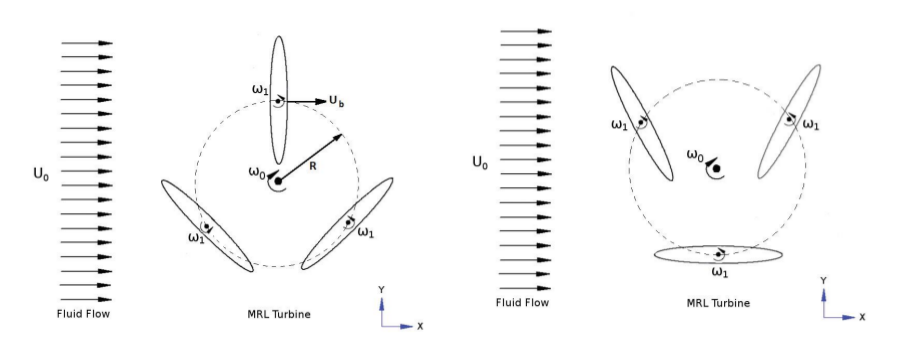
\includegraphics[width=0.8\textwidth]{images/flow.png} 
\end{center}

The flow-blade interaction leads to a drag force that is coming out while the blade is placed in the upper part of the circumferential path and a lift force on each blade located in the lower part of the path.
The resulting torque multplied by the rotating speed will give the generated power of the turbine which, in the end, is our final useful effect. The generated power per turbine is not really high (a few Watts) and this is the reason why the \emph{farm layout}  that Prof. Gavin Tabor showed us at the beginning of the course is used. Many little turbines are placed in a schematic and regular disposition in order to extract a higher power from the tidal stream.
Since from the first raw presentation of the machine we can realise that the mesh will have a relevant importance in the representation and validation of this complex rotating movement. We will deal with a rotating mesh which is progressivly refined closeto the blades, ending with the boundary layers when we are approaching the solid walls of the blades.


\subsection{The data}
The turbine is surrounded by an upcoming water flow set at 1 m/s constant along y axis. 
CAD files were provided by our professor and all the geometry parameters were known.
The in-class workflow has been divided into four little sub-tasks. 

The sub-tasks allowed us to start to get more familiar with the project work and understand the main issues met along the path with the help of the professors. The in-class project started with the raw mesh generation (blockMesh, snappyHexMesh), continued with the preparation of the rotating mesh(AMI files, baffles creation, merge and split procedure), movement of the mesh with the provided motion laws  (real turbine rotation, gif rendering) and finally the set up, running and post processing of the simulation.

\section{In-class work}
\paragraph{In-class workflow}\mbox{}\\
The in-class workflow has been divided into four little sub-tasks. The sub-tasks allowed us to start to get more familiar with the project work and understand the main issues met along the path with the help of the professors. The in-class project started with the raw mesh generation (blockMesh, snappyHexMesh), continued with the preparation of the rotating mesh(AMI files, baffles creation, merge and split procedure), movement of the mesh with the provided motion laws  (real turbine rotation, gif rendering) and finally the set up, running and post processing of the simulation.

\paragraph{Mesh generation}\mbox{}\\
One of the most challenging section of the in-class project was the generation of the raw turbine domain mesh. We have used many different openFoam comands in order to build a complete and exhaustive mesh that must be suitable for the hydraulic problem characteristics.
\\ 
Let's start to present the overall mesh work-flow with all the brief steps evaluation.
\\
\begin{itemize}
\item The scaling of the dimensions and geometry parameters coming from the stl files from millimiters to meters in order to perform correst calculations in the openFoam environment;

\item BlockMesh and SnappyHexMesh for each of the three blades. At this point castellated, snapped and layered mesh have been realized for each blade and we have to join all together;

\item Merging procedure in order to have one complete mesh and the copy of the mesh inside our main environment of the project. We have decided to oparate in this way in order to have a better comunication level in terms of interpolation values among mesh sub-domains. In this way the neighboring cells of different sub-domain are well oriented and aligned. The result is an improvement on the mesh quality controls as non-orthogonality index and skewness coefficient  because we have parallel disposition of cells and they appear as concentric refined layers;

\item Mesh extrusion with the thickness of the 2D domain already given as a geometry parameter equal to the blade width);

\item Wall layer refinement;

\item The first mesh is the 40$\times$120 mesh where the couple of numbers indicates the number of squared and regular cells that are disposed in the y and x direction respectively in the blockMeshDict definition.  
\end{itemize}

Since we deal quite often with different mesh size, in particular during the mesh senitivity analysis, we will call mesh $i$ the mesh with $i$ cells in the y direction, and the cells in the x direction are such a number that let to have squared cells, in order to make the comparison easier and faster to understand.

\paragraph{In-class simulation}\mbox{}\\
In the final part of the in-class project we performed the set up and run of the first raw simulation.
To do so, we have to manage with the boundary conditions of the problem, the turbolence modeling and the numeric schemes. All thease macro-section of the simulation were assigned a priori and the last part of our work is to play with all these parameters and try to understand the influence of each singular changing in the set up on the final result that the turbine must provide.

For the first setup we use the simpler $k\!-\!\varepsilon$ turbolence model respect to more appropriate $k\!-\!\omega \, \text{SST}$.

\subsection{Boundary conditions}
Boundary conditions are referred to the water stream velocity that is investing the machine, the pressure of the water in the stream channel, k, w and nut values.

Our main interest is to focus the first two boundary conditions so velocity and pressure, since the other are maily taken as the default condition for the respective turbolence model.

\paragraph{Patches}\mbox{}\\
Boundary condition are defied over patches so it is important to define that.
\begin{itemize}
\item \emph{Inlet Section} is that from which water comes into the domain moving toward the x direction;
\item \emph{Outlet Section} is where water comes out from the domain;
\item \emph{Front and back faces} are always set to empty since we are dealing with a 2D problem;
\item \emph{Lower wall} is a physical wall that limit the flow;
\item \emph{Upper wall} is a free surface where the flow can slip;
\item \emph{Blades} are physical surfaces that moves inside the domain;
\item \emph{Ami interfaces} are internal patches that allow the communication between moving adiacent cells. All the quantities are set as CyclicAmi.
\end{itemize}


\paragraph{Velocity U}
\begin{itemize}
\item \textbf{Internal field} is uniform at the beginning and it is set to $1\ms$ in the x direction even if in class we have set inlet velocity to $1\ms$ and internal field inited to $0\ms$. We take this decision to make the transition phase faster to limit the simulation time. We are actually interested only in staeady state power so limit the transition let to reduce computational time;
\item \emph{Inlet Section} velocity is fixed to $1\ms$ during all the simulation; 
\item \emph{Outlet Section} velocity is unknown so we have to set it to ZeroGradient boundary condition;
\item \emph{Upper wall} velocity is set to Slip since the fluid can flow in the free stream;
\item \emph{Lower wall} velocity is set to NoSlip which is equivalent to fix the value to zero;
\item \emph{Blades} velocity is set to MovingWallVelocity which is equivalent to NoSlip for moving bodies;
\end{itemize}

\paragraph{Pressure $p$}
\begin{itemize}
\item \textbf{Internal field} is uniform at the beginning and it is set to $0$. 
OpenFoam for incompressible cases works with pressure normalized respect to density. 
Moreover it can manage relative pressures. 
So the value that we set is relative $0 \,\text{bar} \cdot \text{m}^3 / \kg = \m / \s^2$.
\item \emph{Inlet Section} pressure distribution unknown so we set to ZeroGradient; 
\item \emph{Outlet Section} is set to atmospheric ($0 \m / \s^2$) since we assume to be sufficiently far from the blades that pressure is constant;
\item \emph{Upper wall} pressure is set to atmospheric since it is free stream;
\item \emph{Lower wall} pressure is set to ZeroGradient since boundary layer are isobar;
\item \emph{Blades} pressure is set to ZeroGradient since boundary layer are isobar;
\end{itemize}


\section{Mesh sensitivity Analysis}


\section{Numerical Schemes}

\section{Gravitational influence}

\section{Turbolence}

\subsection{Turbolence model}

\paragraph{Laminar}

\paragraph{$k-\varepsilon$ model}

\paragraph{$k-\omega $ SST model}

\subsection{Turbolence intensity}

\section{The domain's sizes}

\section{Results}

\section{Blade speed ratio Analysis}

From what we have seen in mesh sensitivity analysis, the power is quite accurately computed even for a mesh size smaller that that we consider mesh independent.

To obtain a larger number of points from the blade speed ratio analysis we have decided to run most of the simulation with a mesh with 80 cells in the y direction instead of 120. This reduces the number of cells to around 60000 instead of 110000. 
\\Computational time is in this way reduced, but we are not sure that the result is correct.

So we validate just the most significant points with the finer mesh and we compare with the results of the coarser.

We consider that this operating procedure is a proper balance between accuracy and computational cost.

\todo{include fig}

As the mesh sensitivity analysis already highlighted, power is not influenced to much even with this coarser mesh and the difference with the finer mesh is almost negligible.

\subsection{Comparison with experiments}

The trends highlighted by our CFD simulation follow quite accurately that from the real experiments.
The main difference is in terms of absolute value of the power computed. 
This can highlight a difference between the simulated case and the real one, in terms of solidity, ecc \todo 

\section{Conclusion}


















\end{document}